\documentclass[12pt]{book} 

\usepackage{amsmath}
\usepackage{graphicx}
\usepackage{import}
\usepackage{amsfonts}
\usepackage{booktabs}

\setlength{\parindent}{0em}  % sets auto indent at new paragraph to none

\newcommand{\incfig}[1]{%
        \import{./figures/}{#1.pdf_tex}
}

\newcommand{\incimg}[2]{%
       \begin{figure}[h]
               \centering
               \includegraphics[scale = #2]{./figures/#1}
       \end{figure}
}

\title{\coursetitle\linebreak\lecturename}
\author{\\Cain Susko\\ 
           \\ \\ \\
      Queen's University 
    \\School of Computing\\} 

%=-=-=-=-=-title-=-=-=-=-=%
\newcommand{\lecturename}{PCA - Matrix Algebra and Dimensionality Reduction}
\newcommand{\coursetitle}{Linear Data Analysis}
%=-=-=-=-=-#####-=-=-=-=-=%

\begin{document}
\begin{titlepage}
        \maketitle
\end{titlepage}


\section*{a Revisiting the PCA}
this section covers the PCA and will reiterate its axes and scores. 

\paragraph{Data Matrix}
Recall that, within a data matrix, a variable (column) is a real number
with a type. Type has meaning but is not categroical. Thus, an observation is
a ordered list of valuations.

With this clarified we can then take the differences (e.g. from the mean) and the
score as a weighted sum. we shall then gather this data into the matrix
$A \in \mathbb{R}^{m \times n}$

\paragraph{Vector Spaces: Dimensions}
the vector spaced of a full-rank $A \in \mathbb{R}^{m \times n}$ has the 
vector spaces:
\begin{itemize}
        \item Column Space, the general form of the columns within $A$
        \item Row Space, the general form of the rows within $A$
\end{itemize}
Note: the class data generally has a much greater $m$ than $n$: $m >> n$

The dimensionality reduction is done by only using the parts of the right
Singular Martix that are within $\mathbb{R}^n$: 
\[\mathbb{V} \subset \mathbb{R}^n\]

An example of this would be to reduce the grades of 3 quizzes into 1 score.

\paragraph{Terminology}
the PCA of $A$ has the following related variables
\begin{align*}
        M &= A - \vec 1 \bar A &\text{Zero Mean Matrix}\\
        B &= \frac{M^\top M}{m-1} &\text{Covariance Matrix}\\
        \\
        \vec v_1, \vec v_2, ... &= eigenVectors(B) &\text{Loading Vectors}\\
        \\
        \lambda_1, \lambda_2,... &= eigenValues(B) &\text{Latent Variables}
\end{align*}

\section*{b The Scatter Matrix of Variables for PCA}
We will expolre the scatter matrix of the data 

$A \in \mathbb{R}^{m \times n}$ 
and $M = zeroMean(A)$.
The scatter matrix of $A$ would be:
\[S =^{def} M^\top M\]

where $S$ is positive semidifinite.

$S$ has same eigenvectors as the convariance matrix $B$ ($\vec v_1, ...$) and 
has the same scaled eigenvalues as $B$ such that: $(m-1)\lambda_i$.

Thus, $S$ is the \textbf{Weighted Covariance}.

\paragraph{Recall}
The Spectral Throrem where the eigenvectors $\vec v$ of a symmetric matrix 
are a ortho-normal basis for all of the vectors with $m$ entries 
$\mathbb{R}^m$. Thus, the loading vectors $\vec v_i$ are the coordinate axis for
$\mathbb{R}^m$

\paragraph{Algebra}
we get `better' coordinates from using algebra rather than the PCA.
The Geometry that is derived from this algebra can be used to describe the
coordinate axes.

\section*{c PCA as Matrix Approximation}
given the zero mean matrix $M \in \mathbb{R}^{m \times n}$ which has the 
form $M = U\Sigma V^\top$

\paragraph{Rank-p Approximation}
an approximation of the matrix $M$ with rank $p$ is equal to:
\[M = \vec u_1\sigma_1\vec v_1^\top + \vec u_2\sigma_2\vec v_2^\top + ... + \vec u_p\sigma_p\vec v_p^\top\]

Recall that:
\begin{align*}
        \vec v_i^\top \vec v_i &= 1\\
        \vec v_i^\top \vec v_{j \neq i} &= 0
\end{align*}

and thus the PCA Score is:
\[\vec z_1 = M\vec v_1 \equiv \sigma_1 \vec u_1\]
Note: This is the score only for the vector $\vec v_1$.  

\paragraph{Equivalencies}
from this information, we can say that that following values are equivalent
\[\text{First PCA Score }\vec z_1 \equiv \text{ approximation }\sigma_1\vec u_1\]

Additionally, the following approximations are equivalent
\begin{itemize}
        \item Approximate $M$ as a rank-p Matrix using $Z_p = M_pV_p$
        \item Approximate the column space of $M$ as either $Z_p$ or $U_p$
\end{itemize}

thus, if $p=2$ then:
\[Z = [\sigma_1\vec u_1\;\;\; \sigma_2\vec u_2]\]
and equivalently:
\[Z = [\vec u_1\;\;\;\vec u_2]\]

where both score matricies span the space $U_2$.

thus this shows us that approximating the data using the scores $Z$ and 
approximating the data using the left singular vector $U$ result in the same
conclusion as they span the same vector space.

\section*{d PCA as Dimensionality Reduction}
we shall explore Dimensionality Reduction in terms of the PCA.
Using\\ Fisher's Iris Data (petals and sepals) and 2 labels 
(beach-head Iris, everything else)
\begin{figure}[h]
        \centering
        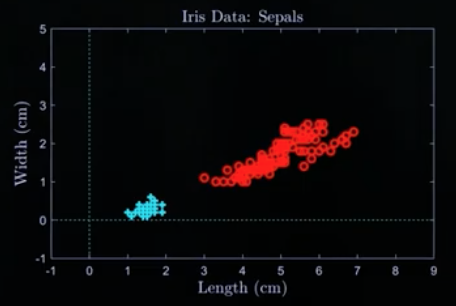
\includegraphics[scale=0.5]{./figures/sepal.png}
        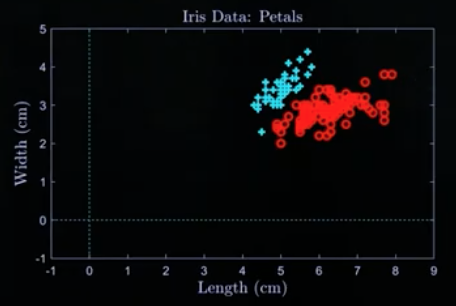
\includegraphics[scale=0.5]{./figures/petal.png}
\end{figure}

we can see that the Sepal Data is aligned along a skewed axis. 

Using PCA we can reduce the dimensionality of this data. 
first, we will define our zero mean matrix as:
\[M = [\vec m_1\vec m_2\vec m_3\vec m_4]\]

where columns 1-4 are the zero mean vectors of: 1; petal length,
2; petal width, 3; sepal length, 4; sepal width.

We will then reduce $M$ using the PCA such that we score each variable within 
$M$ by doing $M\vec v_i$ where the vector $v$ is the $i^{th}$ loading vector; 
thus giving us:
\[\vec S_1, \vec S_2\]

We can then plot these 2 scores like so:
\incimg{PCAscore}{0.5}

and if we then perform the kmeans algorithm with a squared euclidian norm 
 on $M$ we get the corresponding
result:
\incimg{kmeansScore}{0.5}

and we find that kmeans and squared norm does not provide as good of a clustering
PCA (observe the outliers in the kmeans plot)

\section*{Learning Summary}
Students should now be able to:
\begin{itemize}
        \item compute scores of data using the scatter matrix
        \item reduce the dimensionality of the data using the zeor-mean matrix 
                and the loading vectors and apply clustering to the reduced data
        \item interperet some of the results visually
\end{itemize}
\end{document}

